% vim:autoindent:set textwidth=78:
\chapter{Map Composer}
The map composer is a feature that provides improved layout and printing
capabilities. The composer allows you to add elements such as the QGIS map
canvas, legend, scalebar, and text. You can size and position each item and
adjust the properties to create your layout. The result can be printed,
exported as an image, or exported to SVG.

To access the map composer, click on the \textit{Print} button in the toolbar
or choose \textit{Print} from the \textit{File} menu.

\section{Using Map Composer} To use the map composer, first add the layers you
want to print to QGIS. The layes should be rendered and symbolized to your
liking prior to composing the map. 
\begin{figure}[h]
   \begin{center}
   \caption{Map Composer}\label{fig:map_composer_blank}\smallskip
   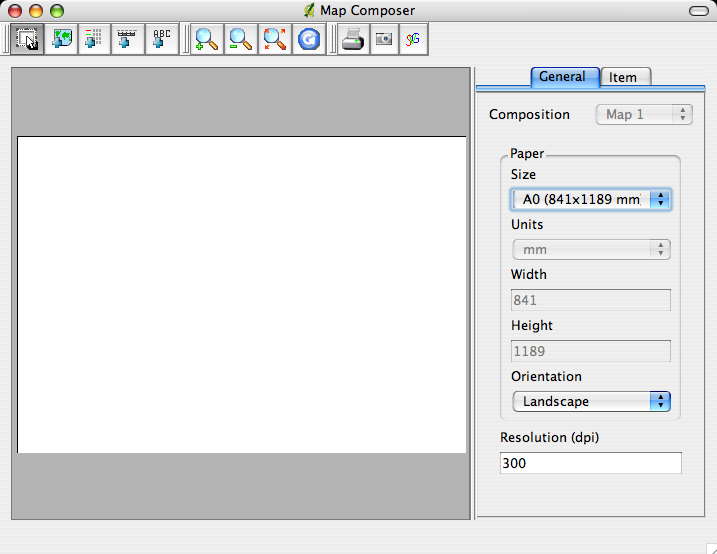
\includegraphics[scale=.70]{qgis_user_guide_images/map_composer_blank}
\end{center}  
\end{figure}
Opening the map composer provides you with a blank canvas to which you can add
the current map view, legend, scalebar, and text. Figure
\ref{fig:map_composer_blank} shows the initial view of the map composer before
any elements are added.

The map composer has two tabs: \textit{General} and \textit{Item}. The
\textit{General} tab allows you to set the paper size, orientation, and
resolution for the map. The \textit{Item} tab displays the properties for the
currently selected map element. By selecting an element on the map (eg.
legend, scalebar, text, etc.) and clicking on the \textit{Item} tab, you can
customize the settings.

You can add multiple elements to the composer. This allows you to have more
than one map view and legend in the composer. Each element has its own
properties and in the case of the map, its own extent.
\subsection{Adding a Map to the Composer}
\parpic[l]{
\includegraphics{qgis_user_guide_images/composer_add_map}}To add the QGIS map canvas to the map composer, click on the \textit{Add a new
map} button in toolbar. Drag a rectangle on the composer canvas to add the
map. You can resize the map later by clicking on the \textit{Select/move item}
button, clicking on the map, and dragging one of the handles in the corner of
the map. With the map selected, you can also resize the map by specifying the
width and height on the Item properties tab.

The map is linked to the QGIS map canvas. If you change the view on the map
canvas by zooming or panning, you can update the map composer view by
selecting the map in composer and clicking on the \textit{Set Extent} button.
You can also change the composer view by specifying a map scale. To set the
view to a specific scale:
\begin{compactenum}
\item Choose \textit{Scale (calculate extent)} from the \textit{Set} drop-down
box
\item Enter the scale denominator in the scale box
\item Press Enter
\end{compactenum} 
\subsection{Adding other Elements to the Composer}
\parpic[l]{
\includegraphics{qgis_user_guide_images/composer_add_legend}}A
legend can be added to the composer canvas and customized to show only the
desired layers. To add a legend, click on the \textit{Add Vector Legend}
button. The legend will be placed on the composer canvas and you can move it
where you like. Click on the \textit{Items} tab to customize the appearance of
the legend, including which layers are shown.
\parpic[l]{
\includegraphics{qgis_user_guide_images/composer_add_scalebar}}To add
a scalebar to the composer, click on the \textit{Add Scalebar} button. Use the
\textit{Item} tab to customize the segment size, number of segments, scalebar
units, size, and font for the scalebar.
\parpic[l]{
\includegraphics{qgis_user_guide_images/composer_add_text}}You can
add text labels to the composer by clicking on the \textit{Add New Label}
button. Use the \textit{Item} tab while the text is selected to customize the
settings or change the default text.

Figure \ref{fig:map_composer_complete} shows the map composer after adding
each type of map element.
\begin{figure}[h]
   \begin{center}
   \caption{Map Composer with map view, legend, scalebar, and text added. The
   map view is currently selected (note the blue rectangles in each corner)}\label{fig:map_composer_complete}\smallskip
   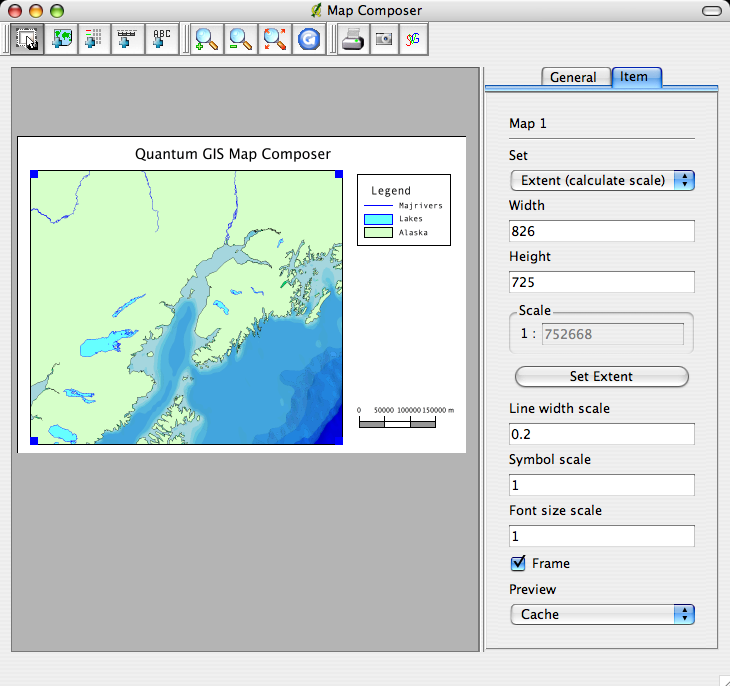
\includegraphics[scale=.70]{qgis_user_guide_images/map_composer}
\end{center}  
\end{figure}
\subsection{Other Features}
The map composer has navigation tools to zoom in and out. To zoom in, click
the zoom in tool. The map composer canvas will be scaled by a factor to 2. Use
the scrollbars to adjust the view to the area of interest. Zooming out works
in a similar fashion.

If you find the view in an inconsistent state, you can use the refresh button
to redraw the map composer canvas.

\subsection{Creating Output}
The map composer allows you to print the map to a printer, export to a PNG, or
export to SVG. Each of these functions is available from the composer toolbar.

